% Gabarit pandoc des corrigés publiés (brut et guidé). Contenu sans marque ni nom de site.
% Compilation : lualatex (latexmk -lualatex).
% Le Markdown reste la source unique : ne pas éditer ce fichier .tex à la main.
\documentclass[11pt,a4paper]{article}

% --- Moteur, polices (Latin Modern) et langue ---------------------------------
\usepackage{iftex}
\ifLuaTeX\else\errmessage{Ce document se compile avec lualatex}\fi
\usepackage{amsmath,amssymb,mathtools}
\usepackage{fontspec}
% mathrm=sym : \mathrm prend ses glyphes dans la police mathématique (ℓ, μ, Ω), comme KaTeX.
\usepackage[math-style=TeX,bold-style=TeX,mathrm=sym]{unicode-math}
% Repli pour les glyphes absents de Latin Modern (indices et exposants Unicode,
% flèches, filets des schémas en texte, symboles) : DejaVu, puis Latin Modern Math
% (ℓ, lettres mathématiques Unicode des légendes).
\directlua{
  luaotfload.add_fallback("repliTexte", {"DejaVuSerif:mode=harf;", "DejaVuSans:mode=harf;", "file:latinmodern-math.otf:mode=harf;"})
  luaotfload.add_fallback("repliMono", {"DejaVuSansMono:mode=harf;", "DejaVuSans:mode=harf;", "file:latinmodern-math.otf:mode=harf;"})
}
\setmainfont{Latin Modern Roman}[RawFeature={fallback=repliTexte}]
\setsansfont{Latin Modern Sans}[RawFeature={fallback=repliTexte}]
\setmonofont{Latin Modern Mono}[RawFeature={fallback=repliMono}]
\setmathfont{Latin Modern Math}
\usepackage[french]{babel}
\frenchsetup{SmallCapsFigTabCaptions=false}

% --- Mise en page --------------------------------------------------------------
\usepackage[a4paper,margin=2.2cm,headheight=14pt,footskip=1.2cm]{geometry}
\usepackage{microtype}
\setlength{\emergencystretch}{4em}
\tolerance=1500
\setlength{\parindent}{0pt}
\setlength{\parskip}{0.55\baselineskip plus 2pt minus 1pt}
\usepackage{xcolor}
% Gris nommés : babel-french rend « ! » actif dans le document.
\definecolor{gris2}{gray}{0.98}
\definecolor{gris3}{gray}{0.97}
\definecolor{gris5}{gray}{0.95}
\definecolor{gris35}{gray}{0.65}
\definecolor{gris40}{gray}{0.60}
\definecolor{gris45}{gray}{0.55}
\definecolor{gris50}{gray}{0.50}
\definecolor{gris55}{gray}{0.45}
\definecolor{gris60}{gray}{0.40}
\definecolor{gris65}{gray}{0.35}
\definecolor{gris70}{gray}{0.30}
\definecolor{gris80}{gray}{0.20}
\definecolor{gris85}{gray}{0.15}
\usepackage{graphicx}
\usepackage{float}
\usepackage{caption}
\captionsetup{font=small,labelformat=empty,justification=centering}
\usepackage{booktabs,longtable,array,multirow,calc}
\usepackage{siunitx}
\sisetup{locale=FR}
\usepackage[version=4]{mhchem}
\usepackage{listings}
\usepackage{fancyhdr}
\usepackage{lastpage}
\usepackage[most]{tcolorbox}
\usepackage{enumitem}
\setlist{nosep,leftmargin=*,topsep=2pt}
\usepackage[hidelinks,unicode]{hyperref}
\usepackage{bookmark}
\hypersetup{pdftitle={X MP — Physique et SI 2026},pdfauthor={Rédigé par IA},pdfcreator={LaTeX},pdfsubject={Corrigé brut}}
\usepackage{xurl}

% --- Pandoc : listes, tableaux, figures ----------------------------------------
\providecommand{\passthrough}[1]{#1}
\providecommand{\tightlist}{\setlength{\itemsep}{0pt}\setlength{\parskip}{0pt}}

\makeatletter
\def\maxwidth{\ifdim\Gin@nat@width>\linewidth\linewidth\else\Gin@nat@width\fi}
\def\maxheight{\ifdim\Gin@nat@height>0.55\textheight 0.55\textheight\else\Gin@nat@height\fi}
\makeatother
\setkeys{Gin}{width=\maxwidth,height=\maxheight,keepaspectratio}
\setcounter{secnumdepth}{-\maxdimen}
\providecommand{\pandocbounded}[1]{#1}
\usepackage{longtable,booktabs,array}

% --- Code (listings) -----------------------------------------------------------
\lstset{
  basicstyle=\ttfamily\small,
  columns=fullflexible,
  keepspaces=true,
  breaklines=true,
  breakatwhitespace=false,
  postbreak=\mbox{\textcolor{gris50}{$\hookrightarrow$}\space},
  frame=single,
  rulecolor=\color{gris35},
  framesep=4pt,
  xleftmargin=5pt,xrightmargin=5pt,
  backgroundcolor=\color{gris3},
  keywordstyle=\bfseries,
  commentstyle=\color{gris65},
  stringstyle=\color{gris80},
  showstringspaces=false,
  tabsize=4,
  extendedchars=true,
  aboveskip=6pt,belowskip=6pt,
}

% --- Macros des corrigés (KaTeX ↔ LaTeX) ---------------------------------------
% Les corrigés sont écrits pour KaTeX : on définit ici ce que KaTeX connaît et
% que LaTeX n'a pas, sans jamais retoucher le Markdown.
\providecommand{\R}{\mathbb{R}}
\providecommand{\N}{\mathbb{N}}
\providecommand{\Z}{\mathbb{Z}}
\providecommand{\Q}{\mathbb{Q}}
\providecommand{\C}{\mathbb{C}}
\providecommand{\dd}{\mathrm{d}}
\providecommand{\llbracket}{\lBrack}
\providecommand{\rrbracket}{\rBrack}
\providecommand{\lBrace}{\lbrace}
\providecommand{\rBrace}{\rbrace}
\providecommand{\Box}{\square}
\providecommand{\Diamond}{\lozenge}
\providecommand{\varnothing}{\emptyset}
\providecommand{\argmax}{\operatorname*{arg\,max}}
\providecommand{\argmin}{\operatorname*{arg\,min}}
\renewcommand{\leq}{\leqslant}
\renewcommand{\geq}{\geqslant}

% Équation hors texte : réduite à la largeur de la ligne si elle déborde.
\newsavebox{\boiteequation}
\newcommand{\equationajustee}[1]{%
  \sbox{\boiteequation}{$\displaystyle #1$}%
  \ifdim\wd\boiteequation>\linewidth
    \[\resizebox{\linewidth}{!}{\usebox{\boiteequation}}\]%
  \else
    \[#1\]%
  \fi}

% --- Encadrés pédagogiques (sobres, lisibles en noir et blanc) -----------------
\tcbset{
  encadre/.style={
    enhanced,breakable,sharp corners,
    colback=white,colframe=gris55,
    boxrule=0.4pt,leftrule=2.2pt,
    left=6pt,right=6pt,top=3pt,bottom=3pt,
    before skip=6pt,after skip=6pt,
    fonttitle=\bfseries\small,coltitle=black,
    attach title to upper,after title={\quad},
    parbox=false,
  }
}
\newtcolorbox{indication}[1]{encadre,colframe=gris45,colback=gris2,title={Indication~#1}}
\newtcolorbox{methode}{encadre,colframe=gris70,title={Méthode}}
\newtcolorbox{piege}{encadre,colframe=gris85,boxrule=0.8pt,leftrule=2.2pt,title={Piège}}
\newtcolorbox{jury}{encadre,colframe=gris60,colback=gris5,title={Jury}}
\newtcolorbox{encadrenote}{encadre,colframe=gris40}

% --- Titres de section ---------------------------------------------------------
\usepackage{titlesec}
\titleformat{\section}{\Large\bfseries}{}{0pt}{}
\titleformat{\subsection}{\large\bfseries}{}{0pt}{}
\titleformat{\subsubsection}{\normalsize\bfseries}{}{0pt}{}
\titlespacing*{\section}{0pt}{14pt plus 4pt minus 2pt}{6pt}
\titlespacing*{\subsection}{0pt}{10pt plus 3pt minus 2pt}{4pt}
\titlespacing*{\subsubsection}{0pt}{8pt plus 2pt minus 2pt}{2pt}

% --- En-tête et pied de page ---------------------------------------------------
\pagestyle{fancy}
\fancyhf{}
\fancyhead[L]{\small\textsc{Corrigé brut} · X MP}
\fancyhead[R]{\small Physique et SI 2026}
\fancyfoot[L]{\footnotesize Corrigé rédigé par IA, non officiel}
\fancyfoot[R]{\footnotesize \thepage\,/\,\pageref*{LastPage}}
\renewcommand{\headrulewidth}{0.4pt}
\renewcommand{\footrulewidth}{0pt}
\fancypagestyle{plain}{\fancyhf{}\fancyfoot[R]{\footnotesize \thepage\,/\,\pageref*{LastPage}}\fancyfoot[L]{\footnotesize Corrigé rédigé par IA, non officiel}\renewcommand{\headrulewidth}{0pt}}

\begin{document}
\thispagestyle{plain}
\begin{center}
  {\small\scshape Corrigé brut}\par\smallskip
  {\LARGE\bfseries X MP — Physique et SI 2026\par}\medskip
  {\large X · MP · Physique et SI · 2026\par}
\end{center}
\vspace{2pt}\hrule\vspace{8pt}

\emph{Corrigé rédigé par IA, non officiel. Signalez toute erreur.}

Épreuve de 4 heures, calculatrice interdite. Deux parties indépendantes : physique (satellites d'étude du Soleil, Q1 à Q17) et sciences de l'ingénieur (déploiement et orientation des panneaux solaires, Q18 à Q37).

\hypertarget{partie-physique-1-communications-entre-le-satellite-et-la-terre}{%
\section{Partie Physique, 1 --- Communications entre le satellite et la Terre}\label{partie-physique-1-communications-entre-le-satellite-et-la-terre}}

\hypertarget{question-1}{%
\subsection{Question 1}\label{question-1}}

\textbf{a.} On étudie une particule de charge \(q\) et de masse \(m\) dans le référentiel terrestre, supposé galiléen. Le plasma est peu dense : on néglige les collisions entre particules. Le poids (\(mg\sim10^{-29}\) N pour un électron) est négligeable devant les forces électromagnétiques, et le champ magnétique terrestre est négligé par hypothèse. La seule force est la force de Lorentz exercée par l'onde. Le principe fondamental de la dynamique s'écrit

\equationajustee{\boxed{m\,\frac{\mathrm d\vec v}{\mathrm dt}=q\left(\vec E(\vec r,t)+\vec v\wedge\vec B(\vec r,t)\right)}}

\textbf{b.} Pour une onde plane, la structure locale donne \(\|\vec B\|\sim\|\vec E\|/c\) (au plus de l'ordre de \(\|\vec E\|/c\) dans le plasma, voir Q3). Le rapport des forces magnétique et électrique vaut donc

\equationajustee{\frac{\|q\,\vec v\wedge\vec B\|}{\|q\,\vec E\|}\lesssim\frac{vB}{E}\sim\frac{v}{c}\ll1 .}

Pour des particules non relativistes, la force magnétique est négligeable et

\equationajustee{\boxed{m\,\frac{\mathrm d\vec v}{\mathrm dt}=q\,\vec E(\vec r,t)}}

De plus, l'amplitude du déplacement des particules, \(qE_0/(m\omega^2)\), est très petite devant la longueur d'onde : on peut évaluer \(\vec E\) à la position moyenne de la particule.

\hypertarget{question-2}{%
\subsection{Question 2}\label{question-2}}

\textbf{a.} En régime harmonique, d'après Q1.b, \(\underline{\vec v}=\dfrac{q}{-\mathrm i\omega m}\underline{\vec E}\) : l'amplitude de la vitesse est proportionnelle à \(|q|/m\). Ions et électrons ont des charges de même valeur absolue \(e\) et des densités égales (\(n_i=n_e\)), donc

\equationajustee{\begin{aligned}
\frac{\|\vec j_i\|}{\|\vec j_e\|}&=\frac{n_i e v_i}{n_e e v_e}\\
&=\frac{m_e}{m_i}\\
&\le\frac{m_e}{m_p}\\
&=\frac{9{,}1\times10^{-31}}{1{,}6\times10^{-27}}\\
&\approx6\times10^{-4}.
\end{aligned}}

\textbf{Les ions, plus de mille fois plus lourds, sont quasi immobiles : seuls les électrons contribuent à la densité de courant.}

\textbf{b.} Pour un électron (\(q=-e\), \(m=m_e\)), avec \(\partial_t\to-\mathrm i\omega\) :

\equationajustee{-\mathrm i\omega m_e\underline{\vec v}=-e\underline{\vec E},}

d'où

\equationajustee{\begin{aligned}
\underline{\vec v}&=\frac{e}{\mathrm i\omega m_e}\underline{\vec E}\\
&=-\mathrm i\,\frac{e}{m_e\omega}\underline{\vec E}.
\end{aligned}}

La densité de courant vaut

\equationajustee{\begin{aligned}
\underline{\vec j}&=-n_e e\,\underline{\vec v}\\
&=\mathrm i\,\frac{n_e e^2}{m_e\omega}\underline{\vec E},
\end{aligned}}

d'où

\equationajustee{\boxed{\underline\sigma=\mathrm i\,\frac{n_e e^2}{m_e\,\omega}=\mathrm i\,\frac{\varepsilon_0\,\omega_p^2}{\omega}}}

avec

\equationajustee{\omega_p^2=\frac{n_e e^2}{\varepsilon_0 m_e}.}

\(\underline\sigma\) est imaginaire pur : courant et champ sont en quadrature, la puissance moyenne cédée par le champ aux électrons est nulle (pas de dissipation).

\hypertarget{question-3}{%
\subsection{Question 3}\label{question-3}}

\textbf{a.} En notation complexe, \(\vec\nabla\to\mathrm i\vec k\) et \(\partial_t\to-\mathrm i\omega\).

\emph{Transversalité.} La conservation de la charge donne \(\omega\underline\rho=\vec k\cdot\underline{\vec j}=\underline\sigma\,\vec k\cdot\underline{\vec E}\), et Maxwell--Gauss donne \(\mathrm i\vec k\cdot\underline{\vec E}=\underline\rho/\varepsilon_0\). En combinant :

\equationajustee{\Big(1-\frac{\omega_p^2}{\omega^2}\Big)\,\vec k\cdot\underline{\vec E}=0 ,}

donc pour \(\omega\neq\omega_p\), \(\vec k\cdot\underline{\vec E}=0\) et \(\underline\rho=0\) : l'onde est transverse.

\emph{Maxwell--Faraday} : \(\mathrm i\vec k\wedge\underline{\vec E}=\mathrm i\omega\underline{\vec B}\), soit \(\underline{\vec B}=\dfrac{\vec k\wedge\underline{\vec E}}{\omega}\).

\emph{Maxwell--Ampère} : \(\mathrm i\vec k\wedge\underline{\vec B}=\mu_0\underline{\vec j}-\mathrm i\omega\mu_0\varepsilon_0\underline{\vec E}\). En reportant \(\underline{\vec B}\) et avec la formule du double produit vectoriel,

\equationajustee{\begin{aligned}
\vec k\wedge(\vec k\wedge\underline{\vec E})&=(\vec k\cdot\underline{\vec E})\vec k-k^2\underline{\vec E}\\
&=-k^2\underline{\vec E},
\end{aligned}}

il vient

\equationajustee{-\frac{\mathrm i k^2}{\omega}\underline{\vec E}=\mu_0\Big(\mathrm i\frac{\varepsilon_0\omega_p^2}{\omega}-\mathrm i\varepsilon_0\omega\Big)\underline{\vec E},}

d'où, avec \(\mu_0\varepsilon_0c^2=1\),

\equationajustee{\boxed{k^2=\frac{\omega^2-\omega_p^2}{c^2}}}

La pulsation particulière, qui annule \(k\), est la \textbf{pulsation plasma}

\equationajustee{\boxed{\omega_p=\sqrt{\frac{n_e e^2}{\varepsilon_0 m_e}}}}

\textbf{b.} Application numérique :

\equationajustee{\begin{aligned}
\omega_p^2&=\frac{10^{12}\times(1{,}6\times10^{-19})^2}{8{,}8\times10^{-12}\times9{,}1\times10^{-31}}\\
&\approx\frac{2{,}6\times10^{-26}}{8{,}0\times10^{-42}}\\
&\approx3{,}2\times10^{15}\ \mathrm{rad^2\,s^{-2}},
\end{aligned}}

soit \(\omega_p\approx5{,}7\times10^{7}\ \mathrm{rad\,s^{-1}}\) et

\equationajustee{\boxed{f_p=\frac{\omega_p}{2\pi}\sim1\times10^{7}\ \mathrm{Hz}\ (\approx 9\ \mathrm{MHz})}}

\textbf{c.} Si l'on déplace en bloc les électrons d'une tranche de plasma par rapport aux ions, la séparation de charges crée un champ électrique de rappel proportionnel au déplacement (\(E=n_e e x/\varepsilon_0\)). Chaque électron obéit alors à \(m_e\ddot x=-\dfrac{n_e e^2}{\varepsilon_0}x\) : il oscille à \(\omega_p\).

\textbf{La fréquence plasma est la fréquence propre des oscillations collectives des électrons autour des ions}, c'est-à-dire le temps de réponse du plasma à une perturbation électrique.

\textbf{d.}

\begin{itemize}
\tightlist
\item
  Si \(\omega<\omega_p\) : \(k^2<0\), donc \(k=\pm\mathrm i/\delta\). La longueur \(\delta=c/\sqrt{\omega_p^2-\omega^2}\) est la profondeur de pénétration. L'onde est \textbf{évanescente}, elle ne transporte pas d'énergie en moyenne et est \textbf{réfléchie} par l'ionosphère. Les électrons suivent le champ assez vite pour l'écranter.
\item
  Si \(\omega>\omega_p\) : \(k\) est réel, l'onde \textbf{se propage} à travers le plasma.
\end{itemize}

\textbf{Le plasma ionosphérique est un filtre passe-haut de fréquence de coupure \(f_p\sim10\) MHz.} Pour communiquer avec un satellite situé au-delà de l'ionosphère, il faut \(f\gg f_p\). À l'inverse, les ondes de fréquence inférieure (ondes courtes, grandes ondes) sont réfléchies et permettent des liaisons terrestres à longue distance.

\hypertarget{question-4}{%
\subsection{Question 4}\label{question-4}}

Pour \(\omega>\omega_p\), \(k=\dfrac1c\sqrt{\omega^2-\omega_p^2}\). En différentiant \(k^2c^2=\omega^2-\omega_p^2\), on obtient \(kc^2\,\mathrm dk=\omega\,\mathrm d\omega\), donc \(v_g=\mathrm d\omega/\mathrm dk=kc^2/\omega\). Avec \(v_\varphi=\omega/k\) :

\equationajustee{\boxed{v_\varphi=\frac{c}{\sqrt{1-\omega_p^2/\omega^2}}>c}}

\equationajustee{\boxed{v_g=c\sqrt{1-\frac{\omega_p^2}{\omega^2}}<c}}

On a \(v_\varphi v_g=c^2\). La vitesse de phase dépasse \(c\) sans contradiction avec la relativité, car elle ne transporte ni énergie ni information. C'est la vitesse de groupe, inférieure à \(c\), qui donne la vitesse de propagation d'un signal.

Quand \(\omega\to\omega_p^+\), \(v_g\to0\) et \(v_\varphi\to+\infty\). Quand \(\omega\gg\omega_p\), \(v_\varphi\simeq v_g\simeq c\) : le plasma se comporte comme le vide.

\hypertarget{question-5}{%
\subsection{Question 5}\label{question-5}}

\textbf{a.} On se limite à \(k\ge0\). La courbe \(k(\omega)=\dfrac1c\sqrt{\omega^2-\omega_p^2}\) n'est définie, avec \(k\) réel, que pour \(\omega\ge\omega_p\).

\begin{itemize}
\tightlist
\item
  Elle part de \((\omega_p,0)\) avec une tangente verticale (\(\mathrm dk/\mathrm d\omega\to+\infty\)).
\item
  Elle est concave et croissante, sous l'asymptote \(k=\omega/c\) (droite passant par l'origine), dont elle s'approche pour \(\omega\gg\omega_p\) : \(k\simeq\dfrac{\omega}{c}-\dfrac{\omega_p^2}{2c\,\omega}\).
\item
  Pour \(\omega<\omega_p\) il n'y a pas de \(k\) réel (zone d'évanescence).
\end{itemize}

\begin{figure}[H]
\centering
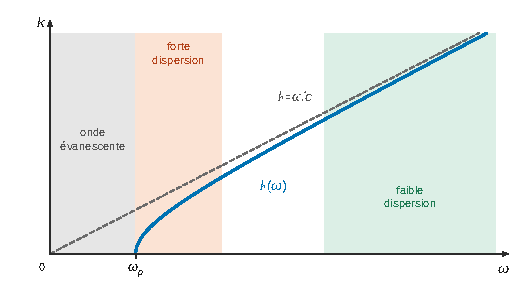
\includegraphics{figures/q05-courbe-dispersion.pdf}
\caption*{Figure 1 --- courbe de dispersion du plasma : coupure en ω\_p, asymptote
k = ω/c, zones de forte et de faible dispersion}
\end{figure}

\emph{Critère.} Un milieu est non dispersif quand \(v_\varphi\) ne dépend pas de \(\omega\). Cela revient à dire que \(k(\omega)\) est une droite passant par l'origine, et alors \(v_g=v_\varphi\).

On mesure la dispersion par l'écart de la courbe à la droite \(k=\omega/c\), ou par la variation de \(v_g\) avec \(\omega\).

\begin{itemize}
\tightlist
\item
  \textbf{Zone de forte dispersion} : \(\omega\) voisin de \(\omega_p\) (quelques \(\omega_p\)). La courbe s'écarte fortement de la droite et \(v_g\) varie très vite.
\item
  \textbf{Zone de faible dispersion} : \(\omega\gg\omega_p\). La courbe se confond avec l'asymptote, et \(v_g\simeq v_\varphi\simeq c\).
\end{itemize}

\textbf{b.} Un signal porteur de données n'est pas monochromatique : c'est un paquet d'ondes de largeur spectrale \(\Delta\omega\) d'autant plus grande que le débit est élevé. Dans un milieu dispersif, les composantes spectrales se propagent à des vitesses de groupe différentes. Le paquet s'étale au cours de la propagation, les impulsions successives se chevauchent (interférence entre symboles) et le signal est déformé. \textbf{La dispersion limite le débit et la fiabilité de la transmission.}

\textbf{c.} La bande Ku (\(10{,}7\) à \(14{,}5\) GHz) vérifie \(f/f_p\sim10^3\) :

\begin{itemize}
\tightlist
\item
  \(f\gg f_p\) : l'onde traverse l'ionosphère sans être réfléchie (Q3.d) ;
\item
  l'écart relatif \(1-v_g/c\simeq\dfrac{f_p^2}{2f^2}\sim3\times10^{-7}\) : la dispersion est négligeable, le signal n'est pas déformé (Q5.a et b) ;
\item
  une porteuse de haute fréquence autorise une large bande passante, donc un débit élevé, et des antennes directives de taille raisonnable.
\end{itemize}

\textbf{La bande Ku garantit une liaison transparente et quasi non dispersive à travers l'ionosphère.} (Au-delà de quelques dizaines de GHz, l'absorption par la vapeur d'eau et la pluie de la basse atmosphère devient gênante, ce qui borne le choix vers le haut.)

\hypertarget{partie-physique-2-points-de-lagrange-et-stabilituxe9}{%
\section{Partie Physique, 2 --- Points de Lagrange et stabilité}\label{partie-physique-2-points-de-lagrange-et-stabilituxe9}}

\textbf{2.1 Étude préliminaire}

\hypertarget{question-6}{%
\subsection{Question 6}\label{question-6}}

\textbf{a.} Le système isolé \{S, T\} a son centre de masse \(O\) fixe dans le référentiel sidéral, qui est galiléen. La Terre décrit un cercle de rayon \(OT=R_T=\dfrac{M_S}{M}R\) à la vitesse angulaire \(\Omega\). Le principe fondamental appliqué à la Terre, projeté sur la direction radiale, donne

\equationajustee{M_T\,\Omega^2\,\frac{M_S}{M}R=\frac{GM_SM_T}{R^2},}

d'où, avec \(M=M_S+M_T\),

\equationajustee{\boxed{\Omega=\sqrt{\frac{GM}{R^3}}}}

C'est la troisième loi de Kepler pour le problème à deux corps.

\textbf{b.} \(T=\dfrac{2\pi}{\Omega}=2\pi\sqrt{\dfrac{R^3}{GM}}\) est la période de révolution commune de S et T autour de leur centre de masse, soit la période de révolution de la Terre autour du Soleil (avec \(M\simeq M_S\) et \(R=1\) UA) :

\equationajustee{\boxed{T\approx1\ \text{an}\approx3\times10^7\ \mathrm s}}

\hypertarget{question-7}{%
\subsection{Question 7}\label{question-7}}

\textbf{a.} Le référentiel \(\mathcal R_\Omega\) tourne à la vitesse angulaire constante \(\vec\Omega=\Omega\vec e_z\). Son axe de rotation \((O,\vec e_\zeta)\) est fixe dans le référentiel galiléen \(\mathcal R_s\). Il n'y a donc pas de terme en \(\dot{\vec\Omega}\), et les forces d'inertie sont :

\begin{itemize}
\tightlist
\item
  la force d'inertie d'entraînement (centrifuge), \(-m\vec\Omega\wedge(\vec\Omega\wedge\overrightarrow{OP})=m\Omega^2\vec r\) pour \(\vec r\) dans le plan \((Oxy)\) ;
\item
  la force de Coriolis, \(-2m\vec\Omega\wedge\vec v\).
\end{itemize}

Le principe fondamental dans \(\mathcal R_\Omega\) s'écrit

\equationajustee{\ddot{\vec r}=-\frac{GM_S}{r_S^3}\vec r_S-\frac{GM_T}{r_T^3}\vec r_T+\Omega^2\vec r-2\Omega\vec e_z\wedge\dot{\vec r}.}

Le terme de Coriolis se projette en

\equationajustee{-2\Omega\vec e_z\wedge(\dot x\vec e_x+\dot y\vec e_y)=2\Omega\dot y\,\vec e_x-2\Omega\dot x\,\vec e_y .}

Les autres termes sont des gradients :

\equationajustee{\begin{aligned}
-\frac{GM_S}{r_S^3}\vec r_S&=\overrightarrow{\mathrm{grad}}\Big(\frac{GM_S}{r_S}\Big)\quad\text{(de \text{même} pour T)},\\
\Omega^2\vec r&=\overrightarrow{\mathrm{grad}}\Big(\frac12\Omega^2r^2\Big).
\end{aligned}}

La projection sur \(\vec e_x\) et \(\vec e_y\) donne

\equationajustee{\begin{aligned}
\ddot x-2\Omega\dot y&=\frac{\partial U}{\partial x},\\
\ddot y+2\Omega\dot x&=\frac{\partial U}{\partial y},
\end{aligned}}

avec la fonction \(U\) explicitée en b. Ce sont bien les équations (2).

\textbf{b.}

\equationajustee{\boxed{U(P)=\frac{GM_S}{r_S}+\frac{GM_T}{r_T}+\frac12\,\Omega^2r^2}}

\emph{Interprétation.} \(-mU\) est l'énergie potentielle dont dérivent les forces de gravitation du Soleil et de la Terre et la force d'inertie d'entraînement (énergie potentielle centrifuge \(-\tfrac12m\Omega^2r^2\)). La force de Coriolis ne dérive pas d'un potentiel mais ne travaille pas : \(U\) est l'opposé d'une énergie potentielle effective par unité de masse dans le référentiel tournant, d'où le nom de pseudo-potentiel.

\hypertarget{question-8}{%
\subsection{Question 8}\label{question-8}}

\textbf{a.} On multiplie la première équation (2) par \(\dot x\), la seconde par \(\dot y\), et on somme. Les termes de Coriolis se compensent (\(-2\Omega\dot x\dot y+2\Omega\dot y\dot x=0\)) :

\equationajustee{\dot x\ddot x+\dot y\ddot y=\frac{\partial U}{\partial x}\dot x+\frac{\partial U}{\partial y}\dot y,}

soit, puisque \(U\) ne dépend pas explicitement du temps dans \(\mathcal R_\Omega\),

\equationajustee{\frac{\mathrm d}{\mathrm dt}\Big(\frac{v^2}{2}\Big)=\frac{\mathrm dU}{\mathrm dt}.}

Donc

\equationajustee{\boxed{C_J=2U-v^2=\text{constante du mouvement}}}

\emph{Interprétation.} \(E=\tfrac12mv^2-mU=-\tfrac m2C_J\) est l'énergie mécanique de P dans le référentiel tournant, en incluant l'énergie potentielle centrifuge. Elle se conserve parce que la force de Coriolis, perpendiculaire à la vitesse, ne travaille pas. La constante de Jacobi est, au facteur \(-m/2\) près, cette énergie mécanique.

\textbf{b.} Comme \(v^2=2U-C_J\ge0\), le point P ne peut occuper que les points où \(U(P)\ge C_J/2\). \textbf{Les zones d'exclusion sont les régions où \(U<C_J/2\).}

Elles sont délimitées par les courbes de vitesse nulle \(U=C_J/2\), qui sont des lignes de niveau de \(U\) comme celles de la figure 2. La valeur de \(C_J\) est fixée par les conditions initiales (position et vitesse dans \(\mathcal R_\Omega\)). Par exemple, si \(C_J/2>U(\mathrm L_1)\), un satellite lancé près de la Terre reste confiné dans la région entourant la Terre, sans pouvoir passer vers le Soleil.

\textbf{2.2 Détermination des positions des points de Lagrange}

\hypertarget{question-9}{%
\subsection{Question 9}\label{question-9}}

\textbf{a.} L'unité de vitesse angulaire est \(u_\Omega=1/u_t\). Or \(1/u_t=2\pi/T=\Omega\), donc \(u_\Omega=\Omega\).

D'après la dimension de \(G\) (\(\mathrm{m^3\,kg^{-1}\,s^{-2}}\)), son unité est

\equationajustee{\begin{aligned}
u_G&=\frac{u_L^3}{u_Mu_t^2}\\
&=\frac{R^3\Omega^2}{M}\\
&=G\quad\text{d'\text{après} Q6.a.}
\end{aligned}}

Donc

\equationajustee{\begin{aligned}
\omega&=\frac{\Omega}{u_\Omega}=\boxed{1},\\
\Gamma&=\frac{G}{u_G}\\
&=\frac{GM}{R^3\Omega^2}\\
&=\boxed{1}.
\end{aligned}}

\textbf{b.} Par définition de \(u_t\),

\equationajustee{\begin{aligned}
\tau&=\frac{t}{u_t}\\
&=\frac{2\pi t}{T}\\
&=\Omega t .
\end{aligned}}

Or l'axe \(\vec e_x\) du référentiel synodique est porté par \(\overrightarrow{ST}\). Il tourne à la vitesse angulaire \(\Omega\) et coïncide avec \(\vec e_\xi\) à \(t=0\). Donc \(\theta=(\vec e_\xi,\vec e_x)=\Omega t\) et

\equationajustee{\boxed{\tau=\theta}}

Le temps adimensionné mesure l'angle dont a tourné le système Soleil--Terre ; un tour complet correspond à \(\tau=2\pi\), soit un an.

\hypertarget{question-10}{%
\subsection{Question 10}\label{question-10}}

Le centre de masse étant à l'origine, S est en \((-\mu_T,0)\) et T en \((\mu_S,0)\), avec \(\mu_S+\mu_T=1\) :

\equationajustee{\begin{aligned}
\rho_S^2&=(\tilde x+\mu_T)^2+\tilde y^2,\\
\rho_T^2&=(\tilde x-\mu_S)^2+\tilde y^2 .
\end{aligned}}

Notons \(f(\rho)=\rho-\dfrac1{\rho^2}\), de sorte que \(\dfrac{\mathrm d}{\mathrm d\rho}\Big(\dfrac1\rho+\dfrac{\rho^2}2\Big)=f(\rho)\). On a \(\dfrac{\partial\rho_S}{\partial\tilde x}=\dfrac{\tilde x+\mu_T}{\rho_S}\) et \(\dfrac{\partial\rho_S}{\partial\tilde y}=\dfrac{\tilde y}{\rho_S}\), et de même pour T. Par dérivation composée :

\equationajustee{\begin{aligned}
\frac{\partial\tilde U}{\partial\tilde x}&=\mu_S\frac{f(\rho_S)}{\rho_S}(\tilde x+\mu_T)+\mu_T\frac{f(\rho_T)}{\rho_T}(\tilde x-\mu_S),\\
\frac{\partial\tilde U}{\partial\tilde y}&=\tilde y\Big[\mu_S\frac{f(\rho_S)}{\rho_S}+\mu_T\frac{f(\rho_T)}{\rho_T}\Big].
\end{aligned}}

Pour un équilibre hors de l'axe (\(\tilde y\neq0\)), la seconde condition donne

\equationajustee{\mu_S\frac{f(\rho_S)}{\rho_S}+\mu_T\frac{f(\rho_T)}{\rho_T}=0 .}

En retranchant \(\tilde x\) fois cette relation à la première, on obtient

\equationajustee{\mu_S\mu_T\Big[\frac{f(\rho_S)}{\rho_S}-\frac{f(\rho_T)}{\rho_T}\Big]=0 .}

Les deux termes sont donc égaux, et chacun est nul puisque leur combinaison à coefficients positifs l'est. Ainsi \(f(\rho_S)=f(\rho_T)=0\) :

\equationajustee{\boxed{\rho_S=\rho_T=1}}

\(\mathrm L_4\) et \(\mathrm L_5\) sont à la distance \(R\) du Soleil et de la Terre : ils forment avec S et T deux \textbf{triangles équilatéraux}. L'égalité \((\tilde x+\mu_T)^2=(\tilde x-\mu_S)^2\) donne \(\tilde x=\dfrac{\mu_S-\mu_T}{2}\), puis \(\tilde y^2=1-\dfrac14\) :

\equationajustee{\boxed{\begin{aligned}
\mathrm L_4\ :\ (\tilde x,\tilde y)&=\Big(\frac12-\mu_T,\ \frac{\sqrt3}2\Big)\\
\mathrm L_5\ :\ (\tilde x,\tilde y)&=\Big(\frac12-\mu_T,\ -\frac{\sqrt3}2\Big)\\
\mathrm L_4,\ \mathrm L_5\ :\ (\rho_S,\rho_T)&=(1,1)
\end{aligned}}}

(\(\mathrm L_4\) est au-dessus de l'axe sur la figure 2, en avance sur la Terre dans le sens de rotation.) On vérifie \(\tilde U(\mathrm L_4)=\tfrac32-\tfrac12\mu_S\mu_T\), soit \(1{,}42\) pour \(\mu_T=0{,}2\), valeur de la légende.

\hypertarget{question-11}{%
\subsection{Question 11}\label{question-11}}

\(\mathrm L_1\) est sur l'axe (\(\tilde y_1=0\)) entre S et T, donc \(-\mu_T<\tilde x_1<\mu_S\) et

\equationajustee{\begin{aligned}
\rho_S&=\tilde x_1+\mu_T,\\
\rho_T&=\mu_S-\tilde x_1,
\end{aligned}}

d'où \(\rho_S+\rho_T=1\).

Sur ce segment, \(\partial\tilde U/\partial\tilde y=0\) par symétrie. De plus \(\dfrac{\partial\rho_S}{\partial\tilde x}=1\) et \(\dfrac{\partial\rho_T}{\partial\tilde x}=-1\). L'équilibre \(\partial\tilde U/\partial\tilde x=0\) s'écrit donc

\equationajustee{\mu_S f(\rho_S)=\mu_T f(\rho_T),}

avec \(\rho_S=1-\rho_T\). On factorise :

\equationajustee{\begin{aligned}
f(1-\rho_T)&=\frac{(1-\rho_T)^3-1}{(1-\rho_T)^2}\\
&=-\frac{\rho_T\,(3-3\rho_T+\rho_T^2)}{(1-\rho_T)^2},\\
f(\rho_T)&=\frac{\rho_T^3-1}{\rho_T^2}\\
&=-\frac{1-\rho_T^3}{\rho_T^2}.
\end{aligned}}

En reportant :

\equationajustee{\mu_S\,\frac{3\rho_T\big(1-\rho_T+\rho_T^2/3\big)}{(1-\rho_T)^2}=\mu_T\,\frac{1-\rho_T^3}{\rho_T^2},}

soit

\equationajustee{\boxed{\frac{\mu_T}{3\mu_S}=\rho_T^3\,\frac{1-\rho_T+\dfrac{\rho_T^2}{3}}{(1-\rho_T)^2(1-\rho_T^3)}}\qquad(5)}

\hypertarget{question-12}{%
\subsection{Question 12}\label{question-12}}

\textbf{a.} Application numérique :

\equationajustee{\begin{aligned}
\alpha&=\frac{\mu_T}{3\mu_S}\\
&=\frac{M_T}{3M_S}\\
&=\frac{6{,}0\times10^{24}}{3\times2{,}0\times10^{30}}\\
&=\boxed{1{,}0\times10^{-6}}
\end{aligned}}

Comme \(\alpha\ll1\), on a \(\rho_T\ll1\), et le membre de droite de (5) vaut \(\rho_T^3\big(1+O(\rho_T)\big)\). Au plus bas ordre, \(\rho_T^3\simeq\alpha\) :

\equationajustee{\boxed{\rho_T\simeq\alpha^{1/3}=1\times10^{-2}}}

(La correction suivante est d'ordre relatif \(\rho_T/3\approx0{,}3\,\%\) ; la racine exacte de (5) vaut \(\rho_T\approx0{,}00997\).)

\textbf{b.}

\equationajustee{\boxed{r_T=\rho_T\,R\simeq10^{-2}\times1{,}5\times10^{11}=1{,}5\times10^{9}\ \mathrm m}}

soit environ \(1{,}5\) million de kilomètres, quatre fois la distance Terre--Lune : c'est la position de SoHO, WIND et SMILE.

\textbf{2.3 Étude de la stabilité des points de Lagrange}

\hypertarget{question-13}{%
\subsection{Question 13}\label{question-13}}

Sur la figure 2, les lignes de niveau ①, ② et ③ se \textbf{croisent} respectivement en \(\mathrm L_1\), \(\mathrm L_2\) et \(\mathrm L_3\). Un point où une ligne de niveau se recoupe est un \textbf{point-col}.

Le long de l'axe S--T, \(\tilde U\) est minimale en ce point : elle tend vers \(+\infty\) de part et d'autre (près d'un astre, ou loin des deux par le terme centrifuge). Dans la direction perpendiculaire, elle est maximale : elle décroît vers \(\mathrm L_4\) et \(\mathrm L_5\), où elle est minimale.

Comme \(E_p=-mU\), l'énergie potentielle présente elle aussi un col : il existe une direction le long de laquelle \(E_p\) est maximale. Un petit écart dans cette direction fait apparaître une force qui éloigne P de l'équilibre.

La force de Coriolis ne peut pas rattraper cela. Avec les notations de Q15, un col donne \(U_{xx}U_{yy}-U_{xy}^2<0\). Le produit des racines en \(\lambda^2\) est alors négatif, d'où une racine \(\lambda\) réelle positive, c'est-à-dire un écart qui croît exponentiellement. \textbf{\(\mathrm L_1\), \(\mathrm L_2\) et \(\mathrm L_3\) sont instables.}

\hypertarget{question-14}{%
\subsection{Question 14}\label{question-14}}

En \(\mathrm L_4\), \(E_p\) est maximale : sans autre force, un satellite écarté de \(\mathrm L_4\) « dévalerait » la colline de potentiel.

Mais dès qu'il prend une vitesse \(\vec v\) dans \(\mathcal R_\Omega\), la force de Coriolis \(-2m\vec\Omega\wedge\vec v\) intervient. Perpendiculaire à la vitesse et d'intensité proportionnelle à \(v\), elle courbe la trajectoire sans modifier l'énergie. Pour \(\vec\Omega\) selon \(+\vec e_z\), elle dévie le mouvement vers la droite.

La chute vers l'extérieur est ainsi convertie en un mouvement de rotation autour de \(\mathrm L_4\), à la manière d'un cyclone qui tourne autour d'une dépression au lieu de la combler. Si la force de Coriolis est assez grande devant la force « répulsive » due au potentiel, la trajectoire reste confinée au voisinage de \(\mathrm L_4\) : c'est une \textbf{stabilité dynamique}, assurée par le mouvement et non par un minimum d'énergie potentielle.

\hypertarget{question-15}{%
\subsection{Question 15}\label{question-15}}

Au point d'équilibre \((x_0,y_0)\), les dérivées premières de \(\tilde U\) sont nulles. Le développement de \(\tilde U\) à l'ordre 2 donne, à l'ordre 1 en \(X\) et \(Y\) :

\equationajustee{\begin{aligned}
\frac{\partial\tilde U}{\partial X}&=U_{xx}X+U_{xy}Y,\\
\frac{\partial\tilde U}{\partial Y}&=U_{xy}X+U_{yy}Y .
\end{aligned}}

Les équations (7) deviennent

\equationajustee{\begin{aligned}
X''&=U_{xx}X+U_{xy}Y+2Y',\\
Y''&=U_{xy}X+U_{yy}Y-2X',
\end{aligned}}

soit

\equationajustee{\begin{pmatrix}X'\\Y'\\X''\\Y''\end{pmatrix}=\mathbf A\begin{pmatrix}X\\Y\\X'\\Y'\end{pmatrix},}

avec

\equationajustee{\boxed{\mathbf A=\begin{pmatrix}0&0&1&0\\0&0&0&1\\U_{xx}&U_{xy}&0&2\\U_{xy}&U_{yy}&-2&0\end{pmatrix}}}

Son polynôme caractéristique est

\equationajustee{\chi_{\mathbf A}(\lambda)=\lambda^4+(4-U_{xx}-U_{yy})\lambda^2+U_{xx}U_{yy}-U_{xy}^2 .}

En \(\mathrm L_4\), les dérivées secondes valent

\equationajustee{\begin{aligned}
U_{xx}&=\tfrac34,\\
U_{yy}&=\tfrac94,\\
U_{xy}&=\tfrac{3\sqrt3}{4}(1-2\mu_T),
\end{aligned}}

ce qui redonne bien l'équation (10).

\hypertarget{question-16}{%
\subsection{Question 16}\label{question-16}}

\textbf{a.} On pose \(\Lambda=\lambda^2\) :

\equationajustee{\Lambda^2+\Lambda+\frac{27}4\mu_T(1-\mu_T)=0 .}

Le mouvement (9) reste borné si et seulement si les quatre \(\lambda_k\) sont imaginaires purs et distincts. En effet, une partie réelle positive donne une divergence exponentielle, et une racine double donne des termes séculaires en \(\tau\,\mathrm e^{\lambda\tau}\). Il faut donc deux racines \(\Lambda\) réelles, strictement négatives et distinctes.

\begin{itemize}
\tightlist
\item
  Elles sont réelles et distinctes si le discriminant est strictement positif : \(1-27\mu_T(1-\mu_T)>0\).
\item
  Leur somme vaut \(-1<0\) et leur produit \(\frac{27}4\mu_T(1-\mu_T)>0\) : si elles sont réelles, elles sont toutes deux négatives.
\item
  Si le discriminant est négatif, les \(\Lambda\) sont complexes conjugués non réels, et parmi les \(\lambda=\pm\sqrt\Lambda\) l'un a une partie réelle positive : instabilité.
\end{itemize}

\equationajustee{\boxed{27\,\mu_T(1-\mu_T)<1\iff\mu_T<\frac{1-\sqrt{23/27}}{2}\approx0{,}0385}}

(\(\mu_T\) désigne la plus petite des deux masses réduites ; c'est le critère de Routh.)

\textbf{b.} Application numérique :

\equationajustee{\begin{aligned}
\mu_T&=\frac{M_T}{M_S+M_T}\\
&\simeq\frac{M_T}{M_S}\\
&=\frac{6{,}0\times10^{24}}{2{,}0\times10^{30}}\\
&=3{,}0\times10^{-6}\ll0{,}04 .
\end{aligned}}

\textbf{La condition est très largement satisfaite : \(\mathrm L_4\) et \(\mathrm L_5\) sont dynamiquement stables pour le système Soleil--Terre}, ce qui est cohérent avec les troyens terrestres observés.

\hypertarget{question-17}{%
\subsection{Question 17}\label{question-17}}

On pose

\equationajustee{\begin{aligned}
\varepsilon&=\frac{27}{4}\mu_T(1-\mu_T)\\
&\simeq\frac{27}{4}\times3{,}0\times10^{-6}\\
&\approx2{,}0\times10^{-5}\ll1 .
\end{aligned}}

Les racines de \(\Lambda^2+\Lambda+\varepsilon=0\) sont alors

\equationajustee{\begin{aligned}
\Lambda_1&\simeq-1+\varepsilon\simeq-1,\\
\Lambda_2&\simeq-\varepsilon\approx-2{,}0\times10^{-5}.
\end{aligned}}

Les solutions sont donc des combinaisons de deux oscillations de pulsations adimensionnées distinctes :

\equationajustee{\begin{aligned}
\omega_1&=\sqrt{-\Lambda_1}\simeq1,\\
\omega_2&=\sqrt{-\Lambda_2}\\
&=\sqrt{\tfrac{27}4\mu_T}\\
&\approx\sqrt{20\times10^{-6}}\\
&\approx4{,}5\times10^{-3}.
\end{aligned}}

Le mouvement est la superposition de deux oscillations de périodes différentes. Les exponentielles de (9) s'entendent en temps adimensionné \(\tau=\Omega t\). Une pulsation adimensionnée \(\omega_k\) correspond donc à la pulsation réelle \(\omega_k\Omega\).

La période correspondante est \(T_k=\dfrac{2\pi}{\omega_k\Omega}=\dfrac{T}{\omega_k}\), avec \(T=1\) an :

\equationajustee{\boxed{\begin{aligned}
T_1&=\frac{T}{\omega_1}\approx1\ \text{an}\\
T_2&=\frac{T}{\omega_2}\approx\frac{1\ \text{an}}{4{,}5\times10^{-3}}\approx2{,}2\times10^{2}\ \text{ans}
\end{aligned}}}

On a bien \(T_2>T_1\) : le satellite décrit une petite boucle annuelle (épicycle) dont le centre dérive lentement autour de \(\mathrm L_4\) avec une période d'environ deux siècles (libration).

\hypertarget{partie-si-2-duxe9ploiement-des-panneaux-solaires}{%
\section{Partie SI, 2 --- Déploiement des panneaux solaires}\label{partie-si-2-duxe9ploiement-des-panneaux-solaires}}

\textbf{2.1 Analyse du mécanisme}

\hypertarget{question-18}{%
\subsection{Question 18}\label{question-18}}

Solides : satellite 0, arbre 1, bras 2, panneaux 3, 4 et 5. Liaisons (« les 3 rotations de l'espace » d'une charnière donnent une liaison \textbf{sphérique}) :

\begin{longtable}[]{@{}
  >{\raggedright\arraybackslash}p{(\columnwidth - 2\tabcolsep) * \real{0.2125}}
  >{\raggedright\arraybackslash}p{(\columnwidth - 2\tabcolsep) * \real{0.7575}}@{}}
\toprule\noalign{}
\begin{minipage}[b]{\linewidth}\raggedright
Solides
\end{minipage} & \begin{minipage}[b]{\linewidth}\raggedright
Liaison
\end{minipage} \\
\midrule\noalign{}
\endhead
\bottomrule\noalign{}
\endlastfoot
0--1 & pivot d'axe \((O_1,\vec x_1)\) \\
1--2 & pivot d'axe \((O_2,\vec z_2)\) (charnière principale) \\
2--3 & sphérique de centre \(J_3\) (charnière passive) et sphérique de centre \(I_3\) (charnière active) \\
3--4 & sphérique de centre \(J_4\) et sphérique de centre \(I_4\) \\
4--5 & sphérique de centre \(J_5\) et sphérique de centre \(I_5\) \\
\end{longtable}

\begin{figure}[H]
\centering
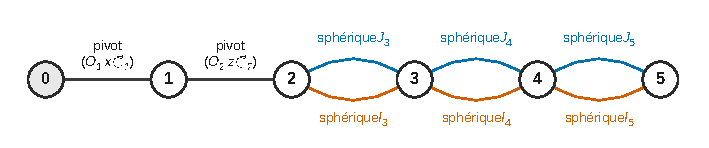
\includegraphics{figures/q18-graphe-liaisons.pdf}
\caption*{Figure 2 --- graphe de liaisons : deux pivots, puis deux sphériques J et
I en parallèle entre solides successifs}
\end{figure}

Entre deux panneaux successifs, il y a deux arcs en parallèle (deux sphériques). Le graphe est une chaîne ouverte dont chaque étage panneau--panneau forme une boucle fermée.

\hypertarget{question-19}{%
\subsection{Question 19}\label{question-19}}

Schéma cinématique en configuration déployée, dessiné dans le plan des panneaux (\(\vec x_1\) horizontal, \(\vec z_2\) vertical) :

\begin{figure}[H]
\centering
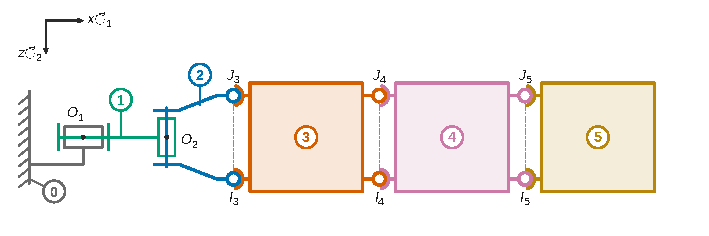
\includegraphics{figures/q19-schema-cinematique.pdf}
\caption*{Figure 3 --- schéma cinématique en configuration déployée, dans le plan
des panneaux}
\end{figure}

\begin{itemize}
\tightlist
\item
  La pivot d'axe \((O_1,\vec x_1)\) (palier lié au bâti 0, arbre 1 à deux épaulements) est dessinée le long de l'axe de l'arbre.
\item
  La pivot d'axe \((O_2,\vec z_2)\) relie l'arbre 1 au bras 2. Son axe \(\vec z_2\) est \textbf{dans le plan des panneaux}, parallèle aux arêtes de charnière.
\item
  Chaque charnière entre deux solides successifs est représentée par deux liaisons sphériques de centres \(J_i\) et \(I_i\), alignées sur l'arête commune, parallèle à \(\vec z_2\) pendant le déploiement.
\end{itemize}

Deux sphériques en parallèle de centres distincts sont équivalentes à une \textbf{pivot d'axe \((J_iI_i)\)}. C'est ce qui justifie la modélisation de la partie 2.2 (pivot d'axe \((O_3,\vec z_0)\) entre 2 et 3). Cette association est hyperstatique de degré 1 (6 inconnues statiques pour 5 mobilités bloquées) : la translation le long de \(J_iI_i\) est bloquée deux fois.

\textbf{2.2 Dynamique du déploiement}

\hypertarget{question-20}{%
\subsection{Question 20}\label{question-20}}

\(\mathcal R_0\) est lié au satellite, qui est en orbite (au voisinage de \(\mathrm L_1\)) et peut tourner sur lui-même. Il est accéléré par rapport au référentiel héliocentrique : \textbf{il n'est pas galiléen}. On peut l'assimiler à un référentiel galiléen pour le déploiement car :

\begin{itemize}
\tightlist
\item
  \textbf{translation} : le satellite est en chute libre. La force d'inertie d'entraînement de translation \(-m\vec a(O_0)\) compense la gravitation, quasi uniforme à l'échelle du mécanisme (quelques mètres). Les termes de marée sont négligeables. Négliger la gravité, comme le fait l'énoncé, n'est cohérent qu'avec cet argument ;
\item
  \textbf{rotation} : la rotation de \(\mathcal R_0\) (orbitale, \(\Omega_{\text{orb}}\approx2\times10^{-7}\ \mathrm{rad\,s^{-1}}\), ou d'attitude, lente et contrôlée) est négligeable à l'échelle des 8 s du déploiement : les forces centrifuge et de Coriolis sont infimes devant les actions des ressorts ;
\item
  \textbf{recul du satellite} : la masse du satellite (de l'ordre de la tonne) est très grande devant celle du bras et des panneaux (quelques kilogrammes). Le mouvement du corps 0 induit par le déploiement est négligeable.
\end{itemize}

\hypertarget{question-21}{%
\subsection{Question 21}\label{question-21}}

Le panneau 3 est un parallélépipède homogène de dimensions :

\begin{itemize}
\tightlist
\item
  \(L\) selon \(\vec x_3\) ;
\item
  \(e\) selon \(\vec y_3\) ;
\item
  \(l\) selon \(\vec z_3\).
\end{itemize}

Les trois plans \((G_3,\vec x_3,\vec y_3)\), \((G_3,\vec y_3,\vec z_3)\) et \((G_3,\vec z_3,\vec x_3)\) sont des plans de symétrie matérielle. Les produits d'inertie sont donc nuls et la matrice est diagonale dans \((\vec x_3,\vec y_3,\vec z_3)\). Par exemple,

\equationajustee{A_3=\int(y^2+z^2)\,\mathrm dm=\frac{m_3}{Lel}\int_{-L/2}^{L/2}\!\!\int_{-e/2}^{e/2}\!\!\int_{-l/2}^{l/2}(y^2+z^2)\,\mathrm dz\,\mathrm dy\,\mathrm dx ,}

avec

\equationajustee{\frac1e\int_{-e/2}^{e/2}y^2\,\mathrm dy=\frac{e^2}{12},}

et de même pour les autres dimensions. On obtient

\equationajustee{\boxed{\begin{aligned}
A_3&=\frac{m_3}{12}\left(e^2+l^2\right)\\
B_3&=\frac{m_3}{12}\left(L^2+l^2\right)\\
C_3&=\frac{m_3}{12}\left(L^2+e^2\right)
\end{aligned}}}

Numériquement :

\equationajustee{\begin{aligned}
A_3&\approx0{,}28\ \mathrm{kg\,m^2},\\
B_3&\approx0{,}86\ \mathrm{kg\,m^2},\\
C_3&\approx0{,}58\ \mathrm{kg\,m^2}.
\end{aligned}}

On a \(C_3\simeq m_3L^2/12\) car \(e\ll L\).

\hypertarget{question-22}{%
\subsection{Question 22}\label{question-22}}

Le problème est plan, \(\vec z_0=\vec z_2=\vec z_3\). Les pivots sont supposées parfaites : elles ne transmettent aucun moment selon leur axe. Le seul moment axial est celui du ressort. Dans la base de \(\mathcal R_2\) :

\equationajustee{\{\mathcal T_{0\to2}\}=\left\{\begin{matrix}X_{02}\,\vec x_2+Y_{02}\,\vec y_2+Z_{02}\,\vec z_2\\ L_{02}\,\vec x_2+M_{02}\,\vec y_2-K_2\,\alpha_2\,\vec z_2\end{matrix}\right\}_{O_2}}

\equationajustee{\{\mathcal T_{2\to3}\}=\left\{\begin{matrix}X_{23}\,\vec x_2+Y_{23}\,\vec y_2+Z_{23}\,\vec z_2\\ L_{23}\,\vec x_2+M_{23}\,\vec y_2-K_3\,\alpha_3\,\vec z_2\end{matrix}\right\}_{O_3}}

Dans l'hypothèse de problème plan, les composantes hors plan \(Z\), \(L\) et \(M\) sont nulles et il reste les deux composantes de résultante, inconnues, et le moment du ressort. Le torseur de 0 sur 2 comprend l'action de la pivot et celle du ressort \(K_2\) ; celui de 2 sur 3 comprend l'action de la pivot et celle du ressort \(K_3\).

\hypertarget{question-23}{%
\subsection{Question 23}\label{question-23}}

\(O_2\) est fixe dans \(\mathcal R_0\). Les vitesses de rotation sont \(\vec\Omega_{2/0}=\dot\alpha_2\vec z_0\) et \(\vec\Omega_{3/0}=(\dot\alpha_2+\dot\alpha_3)\vec z_0\).

\equationajustee{\begin{aligned}
\vec V_{2,0}(G_2)&=\vec V_{2,0}(O_2)+\vec\Omega_{2/0}\wedge\overrightarrow{O_2G_2}\\
&=\dot\alpha_2\vec z_0\wedge\frac L4\vec x_2,
\end{aligned}}

donc

\equationajustee{\boxed{\vec V_{2,0}(G_2)=\frac L4\,\dot\alpha_2\,\vec y_2}}

\(O_3\) est le centre de la pivot entre 2 et 3, donc \(\vec V_{3,0}(O_3)=\vec V_{2,0}(O_3)=\frac L2\dot\alpha_2\vec y_2\), puis

\equationajustee{\boxed{\vec V_{3,0}(G_3)=\frac L2\,\dot\alpha_2\,\vec y_2+\frac L2\,(\dot\alpha_2+\dot\alpha_3)\,\vec y_3}}

soit, dans la base de \(\mathcal R_2\) (avec \(\vec y_3=-\sin\alpha_3\,\vec x_2+\cos\alpha_3\,\vec y_2\)),

\equationajustee{\vec V_{3,0}(G_3)=-\frac L2(\dot\alpha_2+\dot\alpha_3)\sin\alpha_3\,\vec x_2+\frac L2\Big[\dot\alpha_2+(\dot\alpha_2+\dot\alpha_3)\cos\alpha_3\Big]\vec y_2 .}

\hypertarget{question-24}{%
\subsection{Question 24}\label{question-24}}

On dérive dans \(\mathcal R_0\) avec

\equationajustee{\begin{aligned}
\frac{\mathrm d\vec x_2}{\mathrm dt}&=\dot\alpha_2\vec y_2,\\
\frac{\mathrm d\vec y_2}{\mathrm dt}&=-\dot\alpha_2\vec x_2,\\
\frac{\mathrm d\vec y_3}{\mathrm dt}&=-(\dot\alpha_2+\dot\alpha_3)\vec x_3 .
\end{aligned}}

Il vient

\equationajustee{\boxed{\vec a_{2,0}(G_2)=-\frac L4\,\dot\alpha_2^2\,\vec x_2+\frac L4\,\ddot\alpha_2\,\vec y_2}}

\equationajustee{\vec a_{3,0}(G_3)=\frac L2\big(\ddot\alpha_2\vec y_2-\dot\alpha_2^2\vec x_2\big)+\frac L2\Big((\ddot\alpha_2+\ddot\alpha_3)\vec y_3-(\dot\alpha_2+\dot\alpha_3)^2\vec x_3\Big).}

Avec \(\vec x_3=\cos\alpha_3\vec x_2+\sin\alpha_3\vec y_2\) et \(\vec y_3=-\sin\alpha_3\vec x_2+\cos\alpha_3\vec y_2\), on obtient dans \(\mathcal R_2\) :

\equationajustee{\boxed{\vec a_{3,0}(G_3)=\frac L2\Big[-\dot\alpha_2^2-(\dot\alpha_2+\dot\alpha_3)^2\cos\alpha_3-(\ddot\alpha_2+\ddot\alpha_3)\sin\alpha_3\Big]\vec x_2+\frac L2\Big[\ddot\alpha_2-(\dot\alpha_2+\dot\alpha_3)^2\sin\alpha_3+(\ddot\alpha_2+\ddot\alpha_3)\cos\alpha_3\Big]\vec y_2}}

\hypertarget{question-25}{%
\subsection{Question 25}\label{question-25}}

\textbf{Bras 2 en \(O_2\).} La résultante dynamique est \(m_2\vec a_{2,0}(G_2)\). En \(G_2\), la base \((\vec x_2,\vec y_2,\vec z_2)\) est principale et \(\vec\Omega_{2/0}=\dot\alpha_2\vec z_2\). On en déduit \(\vec\delta_{G_2,2/0}=C_2\ddot\alpha_2\vec z_2\). Par transport :

\equationajustee{\vec\delta_{O_2,2/0}=\vec\delta_{G_2,2/0}+\overrightarrow{O_2G_2}\wedge m_2\vec a_{2,0}(G_2),}

avec

\equationajustee{\begin{aligned}
\overrightarrow{O_2G_2}\wedge m_2\vec a_{2,0}(G_2)&=\frac L4\vec x_2\wedge m_2\frac L4\ddot\alpha_2\vec y_2\\
&=m_2\frac{L^2}{16}\ddot\alpha_2\vec z_2 .
\end{aligned}}

D'où

\equationajustee{\boxed{\{\mathcal D_{2/0}\}=\left\{\begin{matrix}m_2\dfrac L4\left(-\dot\alpha_2^2\,\vec x_2+\ddot\alpha_2\,\vec y_2\right)\\[2mm]\Big(C_2+m_2\dfrac{L^2}{16}\Big)\ddot\alpha_2\,\vec z_2\end{matrix}\right\}_{O_2}}}

\textbf{Panneau 3 en \(O_3\).} La résultante dynamique est \(m_3\vec a_{3,0}(G_3)\) (Q24). En \(G_3\), \(\vec\delta_{G_3,3/0}=C_3(\ddot\alpha_2+\ddot\alpha_3)\vec z_2\). Avec \(\overrightarrow{O_3G_3}=\frac L2\vec x_3\) et les produits

\equationajustee{\begin{aligned}
\vec x_3\wedge\vec x_2&=-\sin\alpha_3\,\vec z_2,\\
\vec x_3\wedge\vec y_2&=\cos\alpha_3\,\vec z_2,\\
\vec x_3\wedge\vec y_3&=\vec z_2,
\end{aligned}}

on obtient

\equationajustee{\overrightarrow{O_3G_3}\wedge m_3\vec a_{3,0}(G_3)=m_3\frac{L^2}{4}\Big[(\ddot\alpha_2+\ddot\alpha_3)+\ddot\alpha_2\cos\alpha_3+\dot\alpha_2^2\sin\alpha_3\Big]\vec z_2 ,}

d'où

\equationajustee{\boxed{\{\mathcal D_{3/0}\}=\left\{\begin{matrix}m_3\,\vec a_{3,0}(G_3)\\[1mm]\Big[\Big(C_3+m_3\dfrac{L^2}{4}\Big)(\ddot\alpha_2+\ddot\alpha_3)+m_3\dfrac{L^2}{4}\big(\ddot\alpha_2\cos\alpha_3+\dot\alpha_2^2\sin\alpha_3\big)\Big]\vec z_2\end{matrix}\right\}_{O_3}}}

avec \(m_3\vec a_{3,0}(G_3)\) donnée par Q24.

\hypertarget{question-26}{%
\subsection{Question 26}\label{question-26}}

On cherche deux équations sans inconnues de liaison. On applique le théorème du moment dynamique en projection sur \(\vec z_0\), en un point de l'axe de chaque pivot, et le théorème de la résultante dynamique au panneau 3 pour connaître l'action de 3 sur 2. Gravité négligée, \(\mathcal R_0\) galiléen.

\textbf{Panneau 3 isolé, moment en \(O_3\) sur \(\vec z_0\).} Actions extérieures : la pivot, dont le moment axial est nul en \(O_3\), et le ressort, de moment \(-K_3\alpha_3\). Avec Q25 :

\equationajustee{\Big(C_3+m_3\frac{L^2}{4}\Big)(\ddot\alpha_2+\ddot\alpha_3)+m_3\frac{L^2}{4}\big(\ddot\alpha_2\cos\alpha_3+\dot\alpha_2^2\sin\alpha_3\big)+K_3\,\alpha_3=0\qquad(E_3)}

\textbf{Bras 2 isolé, moment en \(O_2\) sur \(\vec z_0\).} Actions extérieures :

\begin{itemize}
\tightlist
\item
  pivot en \(O_2\) : moment axial nul en \(O_2\) ;
\item
  ressort de la charnière principale : \(-K_2\alpha_2\) ;
\item
  action de 3 sur 2 en \(O_3\) : par les actions réciproques, le moment du ressort vaut \(+K_3\alpha_3\).
\end{itemize}

La résultante \(\vec R_{3\to2}=-\vec R_{2\to3}\) s'obtient par le théorème de la résultante dynamique appliqué à 3, qui ne subit que l'action de 2 : \(\vec R_{2\to3}=m_3\vec a_{3,0}(G_3)\). Son moment en \(O_2\) vaut \(-\big(\overrightarrow{O_2O_3}\wedge m_3\vec a_{3,0}(G_3)\big)\cdot\vec z_0\).

Avec \(\overrightarrow{O_2O_3}=\frac L2\vec x_2\) et Q24,

\equationajustee{\big(\overrightarrow{O_2O_3}\wedge m_3\vec a_{3,0}(G_3)\big)\cdot\vec z_0=\frac L2\,m_3\,\big(\vec a_{3,0}(G_3)\cdot\vec y_2\big),}

d'où

\equationajustee{\Big(C_2+m_2\frac{L^2}{16}\Big)\ddot\alpha_2+m_3\frac{L^2}{4}\Big[\ddot\alpha_2+(\ddot\alpha_2+\ddot\alpha_3)\cos\alpha_3-(\dot\alpha_2+\dot\alpha_3)^2\sin\alpha_3\Big]+K_2\,\alpha_2-K_3\,\alpha_3=0\qquad(E_2)}

Ce sont les deux équations différentielles cherchées. (Isoler l'ensemble \(\{2,3\}\) en \(O_2\) donnerait aussi une équation juste. Elle contiendrait à la fois \(\dot\alpha_2^2\) et \((\dot\alpha_2+\dot\alpha_3)^2\), et aucun terme en \(K_3\alpha_3\). C'est en fait la somme \((E_2)+(E_3)\).)

\hypertarget{question-27}{%
\subsection{Question 27}\label{question-27}}

En regroupant les termes de \((E_2)\) et \((E_3)\) :

\equationajustee{\left\{\begin{aligned}{}&A(\alpha_3)\,\ddot\alpha_2+B(\alpha_3)\,\ddot\alpha_3-C(\alpha_3)\,(\dot\alpha_3+\dot\alpha_2)^2+K_2\,\alpha_2-E\,\alpha_3=0\\
&F\,\ddot\alpha_3+G(\alpha_3)\,\ddot\alpha_2+H(\alpha_3)\,(\dot\alpha_2)^2+K_3\,\alpha_3=0
\end{aligned}\right.}

avec

\equationajustee{\boxed{\begin{aligned}
A(\alpha_3)&=C_2+m_2\frac{L^2}{16}+m_3\frac{L^2}{4}\left(1+\cos\alpha_3\right)\\
B(\alpha_3)&=m_3\frac{L^2}{4}\cos\alpha_3\\
C(\alpha_3)&=m_3\frac{L^2}{4}\sin\alpha_3\\
E&=K_3\\
F&=C_3+m_3\frac{L^2}{4}\\
G(\alpha_3)&=C_3+m_3\frac{L^2}{4}\left(1+\cos\alpha_3\right)\\
H(\alpha_3)&=m_3\frac{L^2}{4}\sin\alpha_3
\end{aligned}}}

Les coefficients d'inertie ne font intervenir que les données demandées par l'énoncé : \(L\), les masses et les moments \(C_2\) et \(C_3\). Le coefficient \(E\) est la raideur \(K_3\), qui intervient dans l'équation du bras par réaction du ressort de la charnière active.

\emph{Contrôle.} On intègre numériquement ce système avec les données de l'énoncé : \(C_3=0{,}58\ \mathrm{kg\,m^2}\), \(\alpha_2(0)=\pi/2\), \(\alpha_3(0)=-\pi\), vitesses initiales nulles. On obtient \(\alpha_2=0\) à \(t=6{,}75\) s, avec \(\alpha_3\approx-50^\circ\) à cet instant. On retrouve la figure 6, ce qui valide les signes.

\textbf{2.3 Validation des résultats}

\hypertarget{question-28}{%
\subsection{Question 28}\label{question-28}}

\textbf{Non.} Les équations (54) décrivent deux pivots libres rappelées par des ressorts. Or un mécanisme bloque chaque pivot lorsque son angle atteint 0. Sur la figure 6, \(\alpha_2\) atteint 0 vers \(t\approx6{,}75\) s puis reste nul. L'angle \(\alpha_3\) continue d'évoluer jusqu'à \(t\approx7{,}7\) s, puis reste nul lui aussi.

Il a fallu une \textbf{résolution par phases}, avec détection de l'instant où un angle s'annule :

\begin{itemize}
\tightlist
\item
  jusqu'à 6,75 s, intégration du système complet (54) ;
\item
  après le verrouillage de la charnière principale, la liaison 0--2 devient un encastrement. La première équation n'est plus valable, car le couple de blocage est une inconnue supplémentaire. On impose \(\alpha_2=\dot\alpha_2=\ddot\alpha_2=0\), et la seconde équation devient \(F\,\ddot\alpha_3+K_3\,\alpha_3=0\). On l'intègre en partant de l'état atteint à 6,75 s ;
\item
  après le verrouillage de la charnière active (\(\alpha_3=0\)), plus aucun mouvement.
\end{itemize}

D'après l'allure de la figure 6, la simulation conserve \(\dot\alpha_3\) continue au moment du blocage de \(\alpha_2\) : elle ne modélise pas le choc.

\hypertarget{question-29}{%
\subsection{Question 29}\label{question-29}}

\begin{itemize}
\tightlist
\item
  \textbf{Durée} : \(\alpha_2\) s'annule à 6,75 s, et \(\alpha_3\) vers \(t\approx7{,}7\) s (le cadre du graphe s'arrête à 8 s, pas la courbe). Le déploiement s'achève en moins de 8 s. \textbf{Critère respecté}, avec une marge faible (environ 0,3 s, soit 4 \%).
\item
  \textbf{Encombrement selon \(\vec y_0\)} : le point le plus éloigné de \(O_2\) est l'extrémité \(M_3\) du panneau. Sur la figure 7, son ordonnée minimale vaut environ \(-0{,}92\) m. Elle est atteinte vers \(x\approx1{,}3\) m, juste avant le point anguleux de la courbe, qui marque le blocage de \(\alpha_2\) à 6,75 s.
\item
  L'ordonnée de \(O_3\) ne dépasse pas \(0{,}6\) m, et l'épaisseur du panneau (\(e/2=1\) cm) ne change rien. On a donc \(|y|\le0{,}92\ \mathrm m<1{,}0\) m : \textbf{critère respecté}, avec une marge d'environ 8 cm.
\end{itemize}

\textbf{Les deux exigences du cahier des charges sont satisfaites par le modèle, avec des marges faibles.}

\hypertarget{question-30}{%
\subsection{Question 30}\label{question-30}}

À \(t=6{,}75\) s, le bras 2 arrive en butée et se verrouille brutalement alors que \(\dot\alpha_2\approx-0{,}47\ \mathrm{rad\,s^{-1}}\) (pente de la figure 6). La vitesse du bras s'annule presque instantanément : c'est un \textbf{choc}.

Il produit des efforts impulsionnels dans la charnière et sur la structure du satellite, ainsi que des \textbf{vibrations} du bras et des panneaux, qui sont en réalité flexibles. Ces vibrations ont été négligées par hypothèse. Le même phénomène se reproduit vers \(7{,}7\) s au verrouillage de la charnière active.

Pour le réduire, on ajoute aux charnières un \textbf{amortisseur} (visqueux ou par courants de Foucault, ou frein de fin de course) qui dissipe l'énergie cinétique avant la butée.

\textbf{Oui, cela peut compromettre le cahier des charges} : l'amortisseur exerce un couple résistant qui ralentit le déploiement. La durée, déjà proche de 8 s, risque de dépasser la limite. Il faut alors raidir les ressorts ou dimensionner l'amortissement pour qu'il n'agisse qu'en fin de course. La trajectoire de \(M_3\) est aussi modifiée, ce qui oblige à revérifier l'encombrement. (À titre d'ordre de grandeur, un choc rigide sur le bras ferait chuter \(\dot\alpha_3\) par conservation du moment cinétique de 3 en \(O_3\), et retarderait sensiblement la fin du déploiement.)

\hypertarget{partie-si-3-orientation-des-panneaux-solaires}{%
\section{Partie SI, 3 --- Orientation des panneaux solaires}\label{partie-si-3-orientation-des-panneaux-solaires}}

\hypertarget{question-31}{%
\subsection{Question 31}\label{question-31}}

Les blocs du schéma de la figure 9, de gauche à droite :

\begin{longtable}[]{@{}
  >{\raggedright\arraybackslash}p{(\columnwidth - 2\tabcolsep) * \real{0.5000}}
  >{\raggedright\arraybackslash}p{(\columnwidth - 2\tabcolsep) * \real{0.5000}}@{}}
\toprule\noalign{}
\begin{minipage}[b]{\linewidth}\raggedright
Emplacement
\end{minipage} & \begin{minipage}[b]{\linewidth}\raggedright
Contenu
\end{minipage} \\
\midrule\noalign{}
\endhead
\bottomrule\noalign{}
\endlastfoot
après le premier comparateur (sortie \(U\)) & gain du comparateur \(K_G\) \\
après le second comparateur & régulateur \(H_v(p)\) \\
bloc suivant (sortie \(U_m\)) & variateur \(K_a\) \\
bloc suivant (sortie \(\Omega_m\)) & moteur \(\dfrac{K_m}{1+\tau_m p}\) \\
bloc suivant (sortie \(\Omega_r\)) & réducteur \(\dfrac1{18}\) \\
dernier bloc (sortie \(\Theta_r\)) & intégrateur \(\dfrac1p\) \\
retour interne, prélevé sur \(\Omega_m\) & codeur incrémental \(K_C\) \\
\end{longtable}

La boucle externe est à \textbf{retour unitaire} (capteur angulaire de gain 1), sans bloc. L'entrée du premier comparateur est \(\Theta_c-\Theta_r\) ; celle du second, \(U-K_C\Omega_m\).

\begin{figure}[H]
\centering
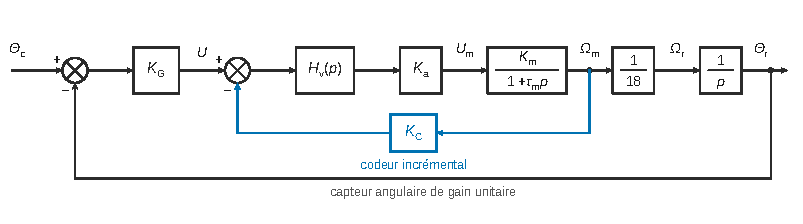
\includegraphics{figures/q31-schema-bloc.pdf}
\caption*{Figure 4 --- schéma de commande complété : boucle de vitesse interne
(codeur K\_C) et boucle de position à retour unitaire}
\end{figure}

\hypertarget{question-32}{%
\subsection{Question 32}\label{question-32}}

Chaîne directe de la boucle interne : \(K_vK_a\dfrac{K_m}{1+\tau_mp}\), retour \(K_C\). D'après la formule de Black,

\equationajustee{\begin{aligned}
H_1(p)&=\frac{K_vK_a\dfrac{K_m}{1+\tau_mp}}{1+K_CK_vK_a\dfrac{K_m}{1+\tau_mp}}\\
&=\frac{K_vK_aK_m}{1+K_CK_vK_aK_m+\tau_mp}\\
&=\frac{K_1}{1+\tau_1p},
\end{aligned}}

avec

\equationajustee{\boxed{\begin{aligned}
K_1&=\frac{K_vK_aK_m}{1+K_CK_vK_aK_m}\\
\tau_1&=\frac{\tau_m}{1+K_CK_vK_aK_m}
\end{aligned}}}

C'est un premier ordre, plus rapide que le moteur seul (\(\tau_1<\tau_m\)).

\hypertarget{question-33}{%
\subsection{Question 33}\label{question-33}}

Pour \(U=U_0/p\), le théorème de la valeur finale donne \(\Omega_m(\infty)=\lim_{p\to0}pH_1(p)\frac{U_0}{p}=K_1U_0\). La consigne de vitesse correspondant à \(U_0\) est \(U_0/K_C\) (vitesse pour laquelle le retour égale \(U_0\)). L'erreur statique vaut

\equationajustee{\begin{aligned}
\varepsilon_s&=\frac{U_0}{K_C}-K_1U_0\\
&=\frac{U_0}{K_C}\,\big(1-K_CK_1\big)\\
&=\frac{U_0}{K_C}\cdot\frac{1}{1+K_CK_vK_aK_m}.
\end{aligned}}

La condition \(\varepsilon_s<0{,}05\,\dfrac{U_0}{K_C}\) impose \(1+K_CK_vK_aK_m>20\), soit

\equationajustee{\boxed{K_v>\frac{19}{K_CK_aK_m}=\frac{19}{1\times1{,}3\times1{,}8}\approx8{,}1}}

(\(K_v\) est sans dimension.)

\hypertarget{question-34}{%
\subsection{Question 34}\label{question-34}}

Le correcteur \(C(p)\) agit sur l'écart de position. On l'insère dans la chaîne directe de la boucle de position, \textbf{entre le gain \(K_G\) du comparateur (sortie : écart en volts) et le comparateur de la boucle de vitesse} :

\begin{figure}[H]
\centering
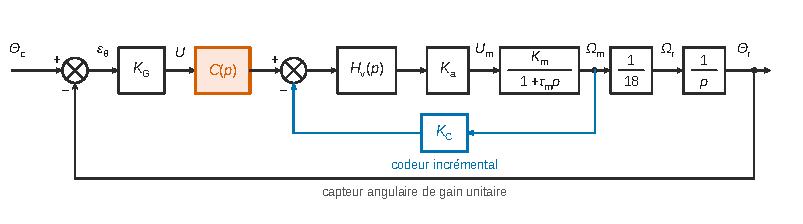
\includegraphics{figures/q34-schema-bloc-correcteur.pdf}
\caption*{Figure 5 --- schéma de commande avec le correcteur C(p) inséré entre
K\_G et la boucle de vitesse}
\end{figure}

Le correcteur se trouve ainsi en amont de la boucle de vitesse et hors de celle-ci.

\hypertarget{question-35}{%
\subsection{Question 35}\label{question-35}}

Avec \(C(p)=K_p\) et la boucle interne réduite à \(H_1(p)\), la fonction de transfert en boucle ouverte est \(\mathrm{FTBO}(p)=\Theta_r/\varepsilon_\theta\) :

\equationajustee{\begin{aligned}
\mathrm{FTBO}(p)&=K_G\,K_p\,H_1(p)\,\frac1{18}\,\frac1p\\
&=\boxed{\frac{K_{BO}}{p\,(1+\tau_1p)}},
\end{aligned}}

avec

\equationajustee{\boxed{K_{BO}=\frac{K_GK_pK_1}{18}}}

Le dénominateur est de degré 2, donc \textbf{ordre 2}. Il y a un pôle nul simple (intégrateur), donc \textbf{classe 1}.

\hypertarget{question-36}{%
\subsection{Question 36}\label{question-36}}

Le retour est unitaire, donc l'écart \(\varepsilon_\theta=\Theta_c-\Theta_r\) s'écrit \(\varepsilon_\theta(p)=\dfrac{\Theta_c(p)}{1+\mathrm{FTBO}(p)}\). Pour un échelon \(\Theta_c=\theta_0/p\), le théorème de la valeur finale donne

\equationajustee{\begin{aligned}
\varepsilon_s&=\lim_{p\to0}p\,\frac{\theta_0/p}{1+\dfrac{K_{BO}}{p(1+\tau_1p)}}\\
&=\lim_{p\to0}\frac{\theta_0\,p(1+\tau_1p)}{p(1+\tau_1p)+K_{BO}}\\
&=\boxed{0}
\end{aligned}}

\textbf{L'erreur statique de position est nulle}, grâce à l'intégrateur en boucle ouverte (classe 1). Le système en boucle fermée est un second ordre à coefficients positifs, donc stable.

\hypertarget{question-37}{%
\subsection{Question 37}\label{question-37}}

Pour une rampe \(\Theta_c=a/p^2\) :

\equationajustee{\begin{aligned}
\varepsilon_v&=\lim_{p\to0}p\,\frac{a/p^2}{1+\dfrac{K_{BO}}{p(1+\tau_1p)}}\\
&=\frac{a}{K_{BO}}\\
&=\frac{18\,a}{K_GK_pK_1}\neq0 .
\end{aligned}}

\textbf{L'erreur de traînage est finie mais non nulle.} Pour l'annuler, il faut une FTBO de classe 2, donc un second intégrateur, placé dans le correcteur. On choisit un \textbf{correcteur à action intégrale de type PI}, \(C(p)=K_p\dfrac{1+T_ip}{T_ip}\), plutôt qu'un intégrateur pur.

Avec un intégrateur pur, la FTBO \(\frac{K}{p^2(1+\tau_1p)}\) donnerait un système bouclé instable. Avec le PI, l'équation caractéristique \(T_i\tau_1p^3+T_ip^2+K_{BO}T_ip+K_{BO}=0\) est stable si et seulement si \(T_i>\tau_1\) (critère de Routh). Le zéro du PI apporte l'avance de phase nécessaire.

\end{document}
